\documentclass[11pt]{exam}
\usepackage{latexsym}
\usepackage{amssymb,amsmath}
\usepackage[pdftex]{graphicx}
\usepackage[top=1in, bottom=1in, left=1in, right=1in]{geometry}
\usepackage{amssymb}
\usepackage{enumitem} 
\usepackage{comment}
\usepackage{mdframed}
%\textwidth=5.5in
%\textheight=8.75in
\pagestyle{headandfoot}
\firstpageheadrule
\runningheadrule
\usepackage{style/header}
\rhead{\name}
\lhead{\class}
\cfoot{Page~\thepage}


\usepackage{latexsym,multirow}
\usepackage{amssymb,amsmath,bm}
\usepackage{graphicx}
\usepackage[color,all,import,arrow]{xy}
\usepackage{booktabs}

%% === bibliography packages ===
\usepackage{natbib}
\bibliographystyle{plainnat}
%% === hyperref options ===
\usepackage{xcolor}
\usepackage[pdftex, bookmarksopen=true, bookmarksnumbered=true,
pdfstartview=FitH, breaklinks=true, urlbordercolor={0 1 0}, citebordercolor={0 0 1}]{hyperref}
\usepackage{colortbl}
\usepackage{subfigure}
\usepackage{subcaption}

%% == tikz
\usepackage{tikz}
\usepackage{inputenc}
\usetikzlibrary{shapes,arrows,trees,fit,positioning,shapes.misc,calc}

% === dcolumn package ===
\usepackage{dcolumn}
\newcolumntype{.}{D{.}{.}{-1}}
\newcolumntype{d}[1]{D{.}{.}{#1}}

% === theorem package ===
\usepackage{theorem}
\theoremstyle{plain}
\theoremheaderfont{\scshape}
\newtheorem{assumption}{Assumption}
\newtheorem{example}{Example}
\newtheorem{definition}{Definition}
\newtheorem{corollary}{Corollary}
\newtheorem{property}{Property}
\newtheorem{proposition}{Proposition}
\newtheorem{theorem}{Theorem}
\newtheorem{remark}{Remark}
\newtheorem{defi}{Definition}
\newtheorem{thm}{Theorem}
\newtheorem{lemma}{Lemma}
\newenvironment{proof}{\paragraph{Proof:}}{\hfill$\square$}

% === some special symbols

\newcommand{\argmax}{\operatornamewithlimits{argmax}}
\newcommand{\argmin}{\operatornamewithlimits{argmin}}
\newcommand{\qed}{\hfill \ensuremath{\Box}}
\newcommand{\ind}{\mbox{$\perp\!\!\!\perp$}}
\newcommand{\nind}{\mbox{$\not\perp\!\!\!\perp$}}
\def\independenT#1#2{\mathrel{\rlap{$#1#2$}\mkern2mu{#1#2}}}
\DeclareMathOperator{\sgn}{sgn}
\DeclareMathOperator{\diag}{diag}
\providecommand{\norm}[1]{\lVert#1\rVert}

\newcommand{\bS}{\bar{s}}
\newcommand{\bs}{\bar{s}}
\newcommand{\N}{\mathbb{N}}
\newcommand{\E}{\mathbb{E}}
\newcommand{\R}{\mathbb{R}}
\newcommand{\bI}{\bm{I}}
\newcommand{\bH}{\bm{H}}
\newcommand{\bM}{\bm{M}}
\newcommand{\bP}{\bm{P}}
\newcommand{\bQ}{\bm{Q}}
\newcommand{\bV}{\bm{V}}
\newcommand{\bU}{\bm{U}}
\newcommand{\cU}{\mathcal{U}}
\newcommand{\bW}{\bm{W}}
\newcommand{\bw}{\bm{w}}
\newcommand{\bepsilon}{\bm{\epsilon}}
\newcommand{\boldeta}{\bm{\eta}}
\newcommand{\bC}{\bm{C}}
\newcommand{\bl}{\bm{\ell}}
\newcommand{\ATT}{\mathrm{ATT}}
\newcommand{\Yone}{Y(1)}
\newcommand{\Yzero}{Y(0)}
\newcommand{\ATE}{\mathrm{ATE}}

\newcommand{\name}{Section 1: Potential Outcomes}
\begin{document}
\noindent
\fbox{%
  \begin{minipage}[t]{\linewidth}
    \class, \term \hfill
    \begin{center}
      \textbf{\Large \name}
    \end{center}
    \emph{\tanames} \hfill
  \end{minipage}
}
\begingroup\small

\section{Causality}

Intuitively, we know why association is not causation. If someone claims that schools giving tablets perform better, we can point out that those schools are typically wealthier and would likely perform better \emph{even without} tablets.\footnote{Running example adapted from Matheus Facure, \emph{Causal Inference for the Brave and True}, “Introduction to Causality”: \url{https://matheusfacure.github.io/python-causality-handbook/01-Introduction-To-Causality.html}.} Let's illustrate this with an example we will use throughout the section.

\subsection{Example: Tablets in Schools}
Let units (here, schools) be indexed by $i=1,\dots,n$. Define the binary treatment
\[
  T_i \in \{0,1\},\quad T_i =
  \begin{cases}
    1 & \text{if school $i$ gives tablets in class},\\
    0 & \text{otherwise.}
  \end{cases}
\]
Let $Y_i \in \R$ denote the observed outcome (e.g., the average test score of school $i$). For each school we define two \emph{potential outcomes}:
\[
  Y_i(0)\ \text{(score if not given tablets)},\qquad Y_i(1)\ \text{(score if given tablets)}.
\]
The central challenge: we never observe the \emph{pair} $\big(Y_i(0),Y_i(1)\big)$ for the same unit (school) at the same time. Indeed, if the treatment (tablets) is given to school $i$ ($T_i=1$), we observe $Y_i(1)$; if no tablets are given ($T_i=0$), we observe $Y_i(0)$. We write this as the observed outcome equals the potential outcome under the received treatment: $Y_i = Y_i(T_i)$. Thus, we observe one potential outcome per unit, not both.
\medskip

\noindent
Suppose (purely for illustration) we could observe \emph{both} potential outcomes for four schools:
\begin{center}
\begin{tabular}{@{}cccccc@{}}
\toprule
$i$ & $Y_i(0)$ & $Y_i(1)$ & $T_i$ & $Y_i$ & $Y_i(1)-Y_i(0)$\\
\midrule
1 & 500 & 450 & 0 & 500 & $-50$\\
2 & 600 & 600 & 0 & 600 & $0$\\
3 & 800 & 600 & 1 & 600 & $-200$\\
4 & 700 & 750 & 1 & 750 & $50$\\
\bottomrule
\end{tabular}
\end{center}

\noindent The (finite-sample) average treatment effect (ATE) is then
\[
\mathrm{ATE} \;=\; \frac{1}{4}\sum_{i=1}^4 (Y_i(1) - Y_i(0)) \;=\; \frac{-50 + 0 - 200 + 50}{4} \;=\; -50,
\]
which indicates that tablets would \emph{lower} students' test scores on average.

\newpage

\section{The Fundamental Problem of Causal Inference}

However, as we eluded to before, for each unit we only only one of $(Y_i(1),Y_i(0))$, never both. In reality the same data would look like:

\begin{center}
\begin{tabular}{@{}ccccc@{}}
\toprule
$i$ & $Y_i(0)$ & $Y_i(1)$ & $T_i$ & $Y_i$\\
\midrule
1 & 500 & --- & 0 & 500\\
2 & 600 & --- & 0 & 600\\
3 & --- & 600 & 1 & 600\\
4 & --- & 750 & 1 & 750\\
\bottomrule
\end{tabular}
\end{center}

\noindent A naive difference in means is
\[
\frac{1}{2}\sum_{i:T_i = 1} Y_i - \frac{1}{2}\sum_{i:T_i = 0} Y_i
= \frac{600+750}{2} - \frac{500+600}{2} \;=\; 125,
\]
which \emph{disagrees} with the causal $\mathrm{ATE}=-50$ above. A naïve comparison of means would suggest tablets improve performance and should be rolled out widely; however, the causal effect is actually negative. The gap reflects selection bias (treated and control schools differ systematically) and underscores why careful causal design and assumptions are essential in public policy, medicine, business and many more.
Mathematically speaking, the phenomena appears because
\[
\frac{1}{4}\sum_{i=1}^n (Y_i(1) - Y_i(0))\neq \frac{1}{2}\sum_{i:T_i = 1} Y_i - \frac{1}{2}\sum_{i:T_i = 0} Y_i
\]
or in super-population terms (we will come back to that),
\[
\E[Y(1)-Y(0)] \neq \E[Y\mid T=1]-\E[Y\mid T=0],
\]
i.e., the causal quantity does not correspond to the statistical one. The main goal of causal inference is to create conditions (or impose assumptions) under which association \emph{becomes} causation by making the groups comparable in their counterfactual outcomes.

\section{Potential Outcomes}
Causal studies ask \emph{what-if} questions: how would $Y$ change if we would set $T$ to a different value?
To formalize this, we use \emph{potential outcomes}. For each unit $i$ and treatment level $t$,
$Y_i(t)$ denotes the outcome that \emph{would} be observed for unit $i$ if, at the time of measurement,
the treatment were set to $t$. Note that $t$ must not need to be $T_i$ and can be different to the observed treatment.

\subsection{Unit-Level Determinism}
We adopt the Neyman-Rubin framework \citep{neyman1923application,rubin1974estimating} of potential outcomes Under this view,
for a fixed unit $i$ the pair of potential outcomes (say for a binary treatment) $\big(Y_i(0),Y_i(1)\big)$ is a \emph{fixed}, non-random attribute of that unit. This is called \emph{unit-level determinism}. This means, when we fix the unit $i$, we also fix all the causal path the unit \emph{could} take under the treatment. However, at the time of treatment, we only ever observe one of the potential causal path, $Y_i = Y_i(T_i)$. The causal ordering is illustrated below:

\begin{center}
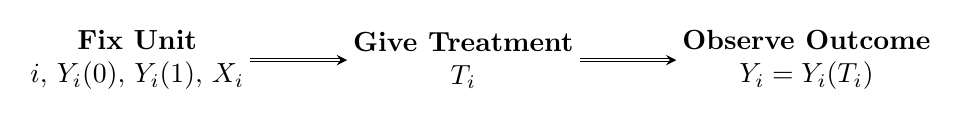
\begin{tikzpicture}[
  node distance=1.3cm,               % tighter spacing between nodes
  every node/.style={align=center,inner sep=1pt}, % tighter padding inside nodes
  >=stealth,                         % arrow tip (works with your current 'arrows' lib)
  doublearrow/.style={->,double, line width=0.4pt, double distance=0.8pt, shorten >=1pt, shorten <=1pt}
]
\node (a) {\textbf{Fix Unit}\\ $i,\,Y_i(0),\,Y_i(1),\,X_i$};
\node (b) [right=of a] {\textbf{Give Treatment}\\ $T_i$};
\node (c) [right=of b] {\textbf{Observe Outcome}\\ $Y_i = Y_i(T_i)$};

\draw[doublearrow] (a) -- (b);
\draw[doublearrow] (b) -- (c);
\end{tikzpicture}
\end{center}
Here $X_i$ denotes pre-treatment covariates (age, race, height, etc.) observed before treatment assignment. Thus potential outcomes are pre-treatment characteristics and not changed by the treatment (but the outcome is).

\subsection{Other Schools of Thought}
Very briefly, let me point out that there are other, perspectives on potential outcomes. For example, \citet{greenland1987interpretation,vanderweele2012stochastic} discuss \emph{stochastic potential outcomes}, where $Y_i(t)$ is random even for a fixed unit $i$ (an approach often used in epidemiology). Others, most prominently \citet{dawid2000causal}, argue that potential outcomes should be avoided altogether (or used only sparingly), since they can never be observed jointly and thus assumptions about them cannot be tested directly. Instead he argues for a \emph{decision-theoretic} approach to causal inference. Finally, the \emph{structural causal model} (SCM) tradition \citep{pearl2009causality} replaces potential outcomes with structural equations and DAGs, using the \emph{do}-operator to formalize interventions. This is a very popular framework, especially in computer science. In practice, these frameworks are often complementary, and when assumptions are aligned they typically agree on the same causal quantities.

\section{Principal Strata}
In the binary case $T_i, Y_i \in \{0,1\}$ it is often useful to classify units by their \emph{principal stratum}:
the potential–outcome pair $\big(Y_i(0),\,Y_i(1)\big)$. In the running example, let $Y_i=1$ indicate that
school $i$’s students meet a proficiency threshold, and $Y_i=0$ indicate that they did not.

\begin{center}
\begin{tabular}{@{}ccl@{}}
\toprule
$\big(Y_i(0),\,Y_i(1)\big)$ & \textbf{Stratum name} & \textbf{Interpretation} \\
\midrule
$(0,0)$ & Never-survivors & Fail regardless of tablets \\
$(0,1)$ & Responders      & Pass only if given tablets \\
$(1,0)$ & Harmed          & Pass only if \emph{not} given tablets \\
$(1,1)$ & Always-survivors& Pass with or without tablets \\
\bottomrule
\end{tabular}
\end{center}

These strata are \emph{principal} because membership is defined by potential outcomes and is therefore invariant to assignment. At the unit level, strata are unobserved since we never see both $Y_i(0)$ and $Y_i(1)$.

\paragraph{Unit-level identifiability.}
From a single unit’s observation $(T_i,Y_i)$ we cannot determine its principal stratum:
\[
\begin{aligned}
T_i=1,\,Y_i=1 &\Rightarrow \text{Responder} \ \text{or}\ \text{Always-survivor} ,\\
T_i=1,\,Y_i=0 &\Rightarrow \text{Harmed} \ \text{or}\ \text{Never-survivor},\\
T_i=0,\,Y_i=1 &\Rightarrow \text{Always-survivor} \ \text{or}\ \text{Harmed},\\
T_i=0,\,Y_i=0 &\Rightarrow \text{Never-survivor} \ \text{or}\ \text{Responder}.
\end{aligned}
\]
Thus the individual effect $\tau_i=Y_i(1)-Y_i(0)$ is not identifiable; we target \emph{average} effects (e.g., ATE) under assumptions.




\section[Identification]{Identification\footnote{Motivated by Prof.\ Matt Blackwell's lecture slides}}

\subsection{Connecting the counterfactual to the observed world}

We distinguish between:
\begin{enumerate}
  \item \emph{Counterfactual} distribution: $(Y_i(1), Y_i(0), T_i, X_i) \sim \mathbb{P}^{\ast}$.
  \item \emph{Observational} distribution: $(Y_i, T_i, X_i) \sim \mathbb{P}$.
\end{enumerate}
Here, $X_i$ denotes observed covariates (extra information we observe about the unit \emph{before} the treatment is given). Causal quantities (e.g., ATE) are functions of $\mathbb{P}^{\ast}$, but our data are sampled from $\mathbb{P}$. Thus, we can learn about $\mathbb{P}^{\ast}$ only through $\mathbb{P}$.

\medskip

\begin{definition}[Identification]
A causal quantity $\tau$ is \emph{identified} if there exists a known map $g$ such that
\[
\tau \;=\; g(\mathbb{P}),
\]
i.e., $\tau$ can be written purely as a function of the observational distribution.
\end{definition}

In general, linking $\mathbb{P}^*$ to $\mathbb{P}$ requires \emph{assumptions} and often we talk about identification strategies like which assumptions allow you to express the causal estimand as a function of observables?



\subsection{Assumptions}
What assumptions let us link the counterfactual world $\mathbb{P}^*$ to the observed world $\mathbb{P}$?
Unless otherwise stated, we will assume:

\begin{itemize}[leftmargin=*]
  \item \textbf{Causal ordering.} $T_i \to Y_i$ (no reverse causality/simultaneity).
  \item \textbf{Stable Unit Treatment Value Assumption (SUTVA).}
    \begin{itemize}[noitemsep,topsep=2pt]
      \item \emph{No interference:} $Y_i(T_1,\dots,T_N)=Y_i(T_i)$; treatments on other units do not affect unit $i$.
      \item \emph{Consistency:} $Y_i = Y_i(T_i)$; the observed outcome equals the corresponding potential outcome.
    \end{itemize}
\end{itemize}

\paragraph{Often also assumed.}
Additional identification assumptions (often needed in observational studies)
\begin{itemize}[leftmargin=*]
  \item \textbf{Randomization / Unconfoundedness}
    \begin{itemize}[noitemsep,topsep=2pt]
      \item \emph{Unconditional (randomized experiments):} $(Y_i(1),Y_i(0)) \;\perp\!\!\!\perp\; T_i$.
      \item \emph{Conditional (observational studies):} $(Y_i(1),Y_i(0)) \;\perp\!\!\!\perp\; T_i \mid X_i$ for a rich set of covariates $X_i$.
    \end{itemize}
  \item \textbf{Positivity / Overlap.} $0<\mathbb{P}(T_i=1\mid X_i)<1$ almost surely (each covariate pattern can, in principle, receive either treatment).
\end{itemize}

\subsection{When Assumptions Fail}

\paragraph{Tablets in Schools}
\begin{itemize}[leftmargin=*]
  \item \emph{Causal ordering:} may fail if higher-scoring schools choose to adopt tablets \emph{because} of prior performance (reverse causality) or if adoption and outcomes are jointly driven by a contemporaneous grant (simultaneity).
  \item \emph{No interference:} may fail if district policies, teacher sharing, or competition create spillovers across schools (one school’s adoption affects others’ outcomes).
  \item \emph{Consistency:} may fail if “tablet use” varies meaningfully (1:1 vs.\ shared devices, different apps, teacher training), so $T_i=1$ does not map to a single well-defined intervention.
  \item \emph{Unconfoundedness:} more plausible only after adjusting for confounders like wealth, baseline scores, teacher quality, and district resources in $X_i$. It \emph{fails} if unobserved factors (e.g., leadership quality, parental involvement) affect both adoption and outcomes even after conditioning. If we only compare schools with and without tablets, richer schools may both adopt tablets and have higher test scores, leading us to overestimate the effect of tablets.
  \item \emph{Overlap:} fails if some strata never/always adopt (e.g., elite private schools always $T=1$, severely underfunded schools always $T=0$), yielding no treated–control overlap for those $X$ values.
\end{itemize}

\paragraph{Flu Shot}
Scenario: Effect of a flu shot ($T$) on days sick ($Y$).

\begin{itemize}[leftmargin=*]
  \item \emph{Causal ordering:} People vaccinate \emph{after} feeling ill $\Rightarrow Y \to T$.
  \item \emph{No interference:} Herd immunity; $Y_i$ depends on others’ $T_j$.
  \item \emph{Consistency:} “Flu shot” has different versions $\Rightarrow T{=}1$ not well-defined.
  \item \emph{Unconfoundedness:}Health-consciousness or access affects both $T$ and $Y$ (selection bias).
  \item \emph{Overlap:} : Some strata always/never vaccinate; no comparable counterfactuals.
\end{itemize}

\begin{example}[ATE]
Assume (i) SUTVA/consistency $Y_i=Y_i(T_i)$, (ii) ignorability $(Y(1),Y(0)) \perp\!\!\!\perp T$, and (iii) positivity $0<\Pr(T=1)<1$.
Then the $\mathrm{ATE}$ can be identified
\begin{alignat*}{2}
\E\!\big[Y(1)-Y(0)\big]
&= \E\!\big[Y(1)\big] - \E\!\big[Y(0)\big]  &\quad& \text{(linearity of expectation)}\\[2pt]
&= \E\!\big[Y(1)\mid T=1\big] - \E\!\big[Y(0)\mid T=0\big]  &\quad& \text{(ignorability \& positivity)}\\[2pt]
&= \E\!\big[Y(T)\mid T=1\big] - \E\!\big[Y(T)\mid T=0\big]  &\quad& \text{(by conditioning)}\\[2pt]
&= \E\!\big[Y\mid T=1\big] - \E\!\big[Y\mid T=0\big]        &\quad& \text{(consistency).}
\end{alignat*}
\emph{Note.} The conditionals $\E[Y(t) \mid T=t]$ and $\E[Y\mid T=t]$ are well-defined only if $\Pr(T=t) > 0$ for $t \in \{0, 1\}$, otherwise we condition on an event of probability zero.
\end{example}

\begin{example}[Non-identified: variance of the individual effect]
Let $\tau_i=Y_i(1)-Y_i(0)$. Even under SUTVA, ignorability, and positivity,
\emph{the variance of the individual treatment effect is not identified}:
\begin{alignat*}{2}
\mathrm{Var}\!\big(Y(1)-Y(0)\big)
&= \mathrm{Var}\!\big(Y(1)\big) + \mathrm{Var}\!\big(Y(0)\big) - 2\,\mathrm{Cov}\!\big(Y(1),Y(0)\big)
\\ 
&= \E\!\big[Y(1)^2\big]+\E\!\big[Y(0)^2\big]-2\,\E\!\big[Y(1)Y(0)\big] - \big(\E[Y(1)]-\E[Y(0)]\big)^2. &&
\end{alignat*}
Randomization identifies the \emph{marginals} ($\E[Y(t)]$, $\mathrm{Var}(Y(t))$), but not the \emph{cross-term}
$\E[Y(1)Y(0)]$ (equivalently $\mathrm{Cov}(Y(1),Y(0))$), since $Y(1)$ and $Y(0)$ are never observed jointly.
Thus $\mathrm{Var}(Y(1)-Y(0))$ is not a function of $\mathbb{P}$ without additional assumptions; at best one can report bounds.
\end{example}

% ---------- Estimation ----------
\section{Estimation}

Identification tells us \emph{what} to estimate, not \emph{how}. Once an estimand is identified, we estimate the corresponding function of $\mathbb{P}$ from data. This is a purely statistical question once identification is established. For instance, a difference-in-means estimator for an identified ATE is
\[
\widehat{\tau}_{\mathrm{ATE}} \;\equiv\; =\frac{1}{n_1}\sum_{i:T_i=1}Y_i-\frac{1}{n_0}\sum_{i:T_i=0}Y_i,
\]
where $n_t=\sum_i \mathbf{1}\{T_i=t\}$ for $t\in\{0,1\}$.

\medskip
\textit{Principle.} Identification comes first; estimation comes second.
Without identification, properties of an estimator are irrelevant.
\endgroup

\bibliography{references}
\end{document}
